\documentclass[10pt,twocolumn]{article}
\usepackage[a4paper,margin=0.62in,columnsep=0.22in]{geometry}
\usepackage[T1]{fontenc}
\usepackage[utf8]{inputenc}
\usepackage{mathptmx}
\usepackage{amsmath}
\usepackage{graphicx}
\usepackage{booktabs}
\usepackage{microtype}
\usepackage[hidelinks]{hyperref}
\usepackage{titlesec}
\usepackage{enumitem}

\titlespacing*{\section}{0pt}{5pt}{2pt}
\titlespacing*{\subsection}{0pt}{4pt}{1pt}
\titleformat*{\section}{\normalsize\bfseries}
\titleformat*{\subsection}{\normalsize\itshape}
\setlength{\parskip}{0pt}
\setlength{\abovecaptionskip}{3pt}
\setlength{\belowcaptionskip}{0pt}
\setlength{\textfloatsep}{6pt}

% Fill in after the GitHub release is archived by Zenodo.
\newcommand{\zenodoDOI}{10.5281/zenodo.XXXXXXX}
\newcommand{\repo}{\url{https://github.com/myaslioglu/tesseract-alife}}

\title{\vspace{-1.2em}\Large\bfseries Tesseract: Self-Replicating Code Organisms\\That Evolve Their Own Attention Layers\vspace{-0.4em}}
\author{Muhsin Murat Ya\c{s}l{\i}o\u{g}lu\\
\small School of Business, Istanbul University, Istanbul, T\"urkiye\\
\small \href{mailto:murat@yaslioglu.com}{murat@yaslioglu.com} \quad ORCID \href{https://orcid.org/0000-0003-2464-5439}{0000-0003-2464-5439}}
\date{\vspace{-1.6em}}

\begin{document}
\maketitle

\begin{abstract}
\noindent Tesseract is an artificial-life system in which every organism is a
file that carries its own genome. In the expression world the genome is an
arithmetic program; in the neural world it is a small transformer with its
weights, architecture and a replay memory. Organisms earn energy on a habitat
drawn from the Mandelbrot set, reproduce with mutation, and may prey on foreign
neighbours, taking their energy and their code or brain. The neural task is
induction, which a one-layer transformer cannot learn (0.14 held-out accuracy
against 1.00 for two layers). We report three results. First, a
function-preserving morph lets the architecture mutate without erasing what
was learned, and three-layer lineages then appear and persist. Second, a kin
rule that looked 24 ancestors deep made predation impossible, because the
whole population descends from one root; limiting kinship to parents and
grandparents restores hunting. Third, against two controls (random survival,
and a single brain trained alone) selection adds nothing measurable on this
task. Code, runs and the original version are public.
\end{abstract}

\section{Introduction}
Tierra and Avida showed that self-replicating programs competing for resources
evolve parasites, cooperation and complex functions \cite{ray,avida,lenski}.
Neuroevolution asks a related question of networks: NEAT grows topologies from
minimal starts \cite{neat}, large-scale and regularized evolution search
architectures while children inherit their parents' weights
\cite{real17,real19}, and population-based training copies trained weights
between workers while it mutates hyperparameters \cite{pbt}. Learning within a
lifetime can also steer evolution \cite{hinton}.

Tesseract joins these lines in a deliberately small setting. An organism is a
file. It reads its own genome, is scored by the environment, and writes mutated
children; in the neural world it carries a transformer \cite{vaswani} that it
trains during its life and passes on. We chose induction because depth is
causal there: copying the token that followed an earlier match needs one head
that tags each position with its predecessor and a second that reads the tag
\cite{elhage,olsson}. A population that loses its second layer should fail.

The contribution is less a success story than an audit: building the controls
changed what we can claim. Section~\ref{sec:system} describes the system,
Section~\ref{sec:results} three findings, and Section~\ref{sec:discussion}
what they imply for evolving learners.

\section{System}\label{sec:system}
\textbf{Organisms.} In the expression world each organism is a Python file
whose genome is one base64 JSON line: an expression of at most 240 characters,
a habitat coordinate, copy fidelity $\mu$, metabolic efficiency $e$, brood
size and diet (the probability of hunting). The file reads itself, evaluates
its expression on six integer lists (target: the sum of squares of the even
entries) and, to reproduce, rewrites its own genome line with character-level
mutations and writes the result to disk as a child. In the neural world the
genome also holds an architecture (width $d$, MLP multiplier, layers $L$,
learning rate), float32 weights and up to 32 replayed examples. Each
generation an organism trains for 800 steps of clipped SGD on fresh batches
plus its memory and is scored on 128 sequences it has never seen.
Backpropagation is hand-written in NumPy and matches finite differences to
$4\times10^{-10}$. A standard-library-only organism ($d=8$, 52 times slower)
trains and rewrites itself on any machine with Python.

\textbf{Habitat and energy.} Fertility at $(c_r,c_i)$ is the Mandelbrot escape
time scaled to $[0.35,2.75]$, or 0.30 inside the set, so only the boundary is
rich \cite{mandelbrot}; the iteration cap grows by three per generation.
Energy changes by $p f e^{1/2}-6e^2$ for score $p$ and fertility $f$, which
puts the best efficiency at $e^*=(pf/24)^{2/3}$ with no bound on $e$. The
$K/\bar b$ organisms with the most energy survive ($\bar b$ is the mean brood)
and split their energy among their children.

\textbf{Task.} Eight distinct tokens from a vocabulary of 12 are followed by a
repeat of one of them; the target is the token that came after it. After 800
steps a two-layer model ($d=32$) reaches 1.00 held-out accuracy and a
one-layer model 0.14, the score of copying a random earlier token (1/7).

\textbf{Morph.} Architecture mutates in 2\% of births ($L\pm1$, MLP multiplier
$\pm1$, or a new $d$). Instead of reinitialising, \texttt{morph()} embeds the
old weights. An inserted block has $W_o=W_2=b_2=0$ and is therefore the
identity on the residual stream, as with zero-initialised residual branches
\cite{net2net,rezero}; new width reads from the stream but writes zeros into
it, and $W_q$ is scaled by $\sqrt{d'/d}$ to keep the attention temperature.
Growth leaves every logit unchanged ($|\Delta|<10^{-15}$); shrinking discards
weights.

\textbf{Predation.} With probability set by its diet gene an organism hunts:
it pays 4 energy, takes 45\% of a neighbour's energy, adopts the neighbour's
expression or whole brain, and forages at 60\% for that generation. Prey must
not be kin, defined as sharing a parent or grandparent \cite{hamilton}, and
must be foreign: a different expression, or a relative weight distance of at
least 0.10 (measured: siblings 0.06, second cousins 0.12, unrelated brains
1.4).

\textbf{Containment.} Expressions must pass an AST whitelist (arithmetic,
comparisons, comprehensions, calls to nine built-ins; no attributes, imports
or assignment) and run in a subprocess with a 6\,s timeout and a 512\,MB
address-space limit, so \texttt{c*10**9} dies of \texttt{MemoryError} and its
owner starves. Organisms have no network access.

\section{Results}\label{sec:results}
\subsection{The predator that never ate}
The original rule required prey to share no ancestor among the last 24 lineage
entries. Every organism descends from one root whose identifier stays in every
lineage for 24 generations, so no legal prey can exist before then, whatever
the genotypes look like; afterwards a population of $N\approx12$ coalesces
within $O(N)$ generations \cite{kingman}, so most pairs remain kin. Re-running
the original code gave zero hunts in 34 generations of the expression world
and in 12 of the neural world, and the earlier refusals had been read as a
sign of clonality. With kinship limited to two generations the neural world
made ?? hunts per 12-generation run (5 seeds), and an 80-generation expression
run made 62 hunts while the diet gene rose from 0.05 to 0.40.

\subsection{A layer born without forgetting}
Before the morph, any change of shape reinitialised the brain, so a mutant
raced parents with thousands of training steps and starved; a 2$\to$1 layer
mutation also crashed the simulation, because leftover weights passed the
shape check. ``Layers never dropped below two'' therefore measured a handicap,
not a necessity. With the morph, three-layer brains appeared in ?? of 5 runs
and persisted (seed 7: born in generation 6, three of the twelve newborns at
the end). On a task that two layers already solve, the third layer looks close
to neutral.

\subsection{Selection is not yet doing the work}
Figure~\ref{fig:arms} compares the full world (\emph{evolve}) with the same
world under random survival (\emph{drift}) and with a single brain trained
alone, without mutation or selection (\emph{train}). ??

\begin{figure}[t]
\centering
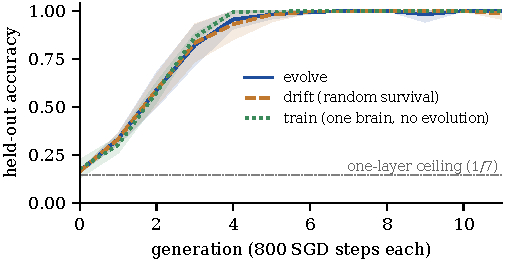
\includegraphics[width=\columnwidth]{fig_arms.pdf}
\caption{Mean held-out accuracy of the population per generation, five seeds
(line: mean; band: $\pm1$ s.d.). K = 12, 800 SGD steps per generation.}
\label{fig:arms}
\end{figure}

\section{Discussion}\label{sec:discussion}
Tesseract's lineages are Lamarckian: a child starts where its parent's
training ended, as in population-based training \cite{pbt}. When gradient
descent can solve the task inside one lineage within a few generations,
selection has nothing left to choose. Evolution should matter when a single
learner cannot get there alone: tasks that shift, competing niches, or a
compute budget too small for one lineage. Two lessons travel beyond this
system. A kin-recognition window longer than the population's coalescence time
makes everyone kin. And an architecture search that reinitialises its mutants
measures the cost of forgetting, not the value of the architecture.

\textbf{Limitations.} Populations are small ($K=12$); the neural results come
from five seeds and one task, the expression-world numbers from single runs;
retention is measured on examples the organism trained on.

\textbf{Code and data.} \repo, archived at Zenodo
(\href{https://doi.org/\zenodoDOI}{doi:\zenodoDOI}). Tag \texttt{v0} keeps the
original code, and every number above can be regenerated with the commands in
the README.

\begingroup
\footnotesize
\setlength{\itemsep}{0pt}
\begin{thebibliography}{99}
\setlength{\itemsep}{0pt}
\setlength{\parskip}{0pt}
\bibitem{ray} T.~S. Ray. An approach to the synthesis of life. In C.~G. Langton et al. (eds.), \emph{Artificial Life II}, pp.~371--408. Addison-Wesley, 1991.
\bibitem{avida} C.~Ofria and C.~O. Wilke. Avida: a software platform for research in computational evolutionary biology. \emph{Artificial Life}, 10(2):191--229, 2004.
\bibitem{lenski} R.~E. Lenski, C.~Ofria, R.~T. Pennock, and C.~Adami. The evolutionary origin of complex features. \emph{Nature}, 423:139--144, 2003.
\bibitem{neat} K.~O. Stanley and R.~Miikkulainen. Evolving neural networks through augmenting topologies. \emph{Evolutionary Computation}, 10(2):99--127, 2002.
\bibitem{real17} E.~Real, S.~Moore, A.~Selle, S.~Saxena, Y.~L. Suematsu, J.~Tan, Q.~V. Le, and A.~Kurakin. Large-scale evolution of image classifiers. In \emph{ICML}, PMLR 70:2902--2911, 2017.
\bibitem{real19} E.~Real, A.~Aggarwal, Y.~Huang, and Q.~V. Le. Regularized evolution for image classifier architecture search. In \emph{AAAI}, 33(1):4780--4789, 2019.
\bibitem{pbt} M.~Jaderberg et al. Population based training of neural networks. arXiv:1711.09846, 2017.
\bibitem{hinton} G.~E. Hinton and S.~J. Nowlan. How learning can guide evolution. \emph{Complex Systems}, 1(3):495--502, 1987.
\bibitem{vaswani} A.~Vaswani et al. Attention is all you need. In \emph{NeurIPS}, 30, 2017.
\bibitem{elhage} N.~Elhage et al. A mathematical framework for transformer circuits. \emph{Transformer Circuits Thread}, 2021.
\bibitem{olsson} C.~Olsson et al. In-context learning and induction heads. arXiv:2209.11895, 2022.
\bibitem{mandelbrot} B.~B. Mandelbrot. \emph{The Fractal Geometry of Nature}. W.~H. Freeman, 1982.
\bibitem{net2net} T.~Chen, I.~Goodfellow, and J.~Shlens. Net2Net: accelerating learning via knowledge transfer. In \emph{ICLR}, 2016.
\bibitem{rezero} T.~Bachlechner, B.~P. Majumder, H.~H. Mao, G.~W. Cottrell, and J.~McAuley. ReZero is all you need: fast convergence at large depth. In \emph{UAI}, PMLR 161:1352--1361, 2021.
\bibitem{hamilton} W.~D. Hamilton. The genetical evolution of social behaviour.~I. \emph{J. Theoretical Biology}, 7(1):1--16, 1964.
\bibitem{kingman} J.~F.~C. Kingman. The coalescent. \emph{Stochastic Processes and their Applications}, 13(3):235--248, 1982.
\end{thebibliography}
\endgroup

\end{document}
